% Methodology section

\subsection{Operads}

A large class of mathematical theories consists of three ingredients:
\begin{enumerate}
  \item A collection of objects.
  \item A collection of morphisms between these objects.
  \item A notion of composition of these morphisms.
\end{enumerate}

The most well-known example of this pattern is arithmetic, where the objects are numbers, the morphisms are functions (addition, multiplication, etc.), and the composition is the usual function composition. All fields such as real numbers, complex numbers, and vector spaces can be described in this way.

As we go up the hierarchy of mathematics, we find more and more examples of this pattern. For example, in topology, the objects are topological spaces, the morphisms are continuous functions, and the composition is the usual function composition. Groups and family (magma, monoid, group, ring, field) are also examples of this pattern. Category theory is a generalization of this pattern, where the objects are categories, the morphisms are functors, and the composition is the usual functor composition.

Operads are a generalization of this pattern, where the objects are operations, the morphisms are operations of different arities, and the composition is a more general form of function composition. Operads provide a framework for studying algebraic structures that arise in various areas of mathematics, including topology, algebra, and category theory.

Operads consists of:

\begin{enumerate}
  \item A collection of operations of different arities.
  \item A notion of composition of these operations.
  \item The composition operations obey certain conditions - associativity and unitality.
\end{enumerate}

\subsubsection{Formal Definition}

Consider a set $\mathbb{X}$, and an integer $n \in \mathbb{N}$.

An Operad, $\mathbb{P}$, is defined as a set of n-ary operations, where each operation $f$ has the signature $\mathbb{X}^n \to \mathbb{X}$:

\begin{equation}
  \mathbb{P}(n) = \{f: \mathbb{X}^n \to \mathbb{X}\}
\end{equation}

where $\mathbb{X}^n$ is the cartesian product of $\mathbb{X}$ with itself $n$ times, i.e.

\begin{equation}
  \mathbb{X}^n = \mathbb{X} \times \mathbb{X} \times \ldots \times \mathbb{X}
\end{equation}

i.e. all of these functions $f$ take in $n$ arguments from $\mathbb{X}$ and return a single element from $\mathbb{X}$.

\begin{figure}[h]
\centering
    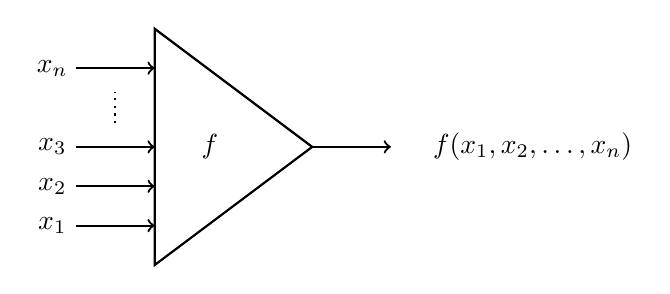
\begin{tikzpicture}
    % Draw the triangle with vertical left edge
    \draw[thick, fill=white] (0,0) -- (0,3) -- (2,1.5) -- cycle;

    % Draw input arrows
    \draw[->, thick] (-1,0.5) -- (0,0.5);
    \draw[->, thick] (-1,1) -- (0,1);
    \draw[->, thick] (-1,1.5) -- (0,1.5);
    \draw[dotted, thick] (-0.5,1.8) -- (-0.5,2.2);
    \draw[->, thick] (-1,2.5) -- (0,2.5);

    % Draw output arrow
    \draw[->, thick] (2,1.5) -- (3,1.5);

    % Add labels
    \node at (0.7,1.5) {$f$};
    \node at (-1.3,0.5) {$x_1$};
    \node at (-1.3,1) {$x_2$};
    \node at (-1.3,1.5) {$x_3$};
    \node at (4.8,1.5) {$f(x_1,x_2,\ldots,x_n)$};
    \node at (-1.3,2.5) {$x_n$};
\end{tikzpicture}
\end{figure}

If we have a bunch of these sets of functions $\mathbb{P}(k_i)$ for each $k_i \in \mathbb{N}$, then we can define a composition operation $\circ$ for these operations as follows:

Let $f_i \in \mathbb{P}(k_i)$ be an operation that takes in $k_i$ arguments from $\mathbb{X}$ and returns a single element from $\mathbb{X}$. We can take n numbers of such operations and use their outputs as inputs to another operation $f \in \mathbb{P}(n)$, which takes in $n$ arguments from $\mathbb{X}$ and returns a single element from $\mathbb{X}$. The composition operation $\circ$ is defined as:

\begin{equation}
    \mathbb{P}(n) \times ( \mathbb{P}(k_1) \times \mathbb{P}(k_2) \times \ldots \times \mathbb{P}(k_n) ) \to \mathbb{P}(k_1 + k_2 + \ldots + k_n)
\end{equation}

\begin{equation}
    f, (f_1, f_2, \ldots, f_n) \mapsto f \circ (f_1, f_2, \ldots, f_n)
\end{equation}

where $f \circ (f_1, f_2, \ldots, f_n) \in \mathbb{P}(k_1 + k_2 + \ldots + k_n)$ is defined as the following diagram:

\begin{figure}[h]
\centering
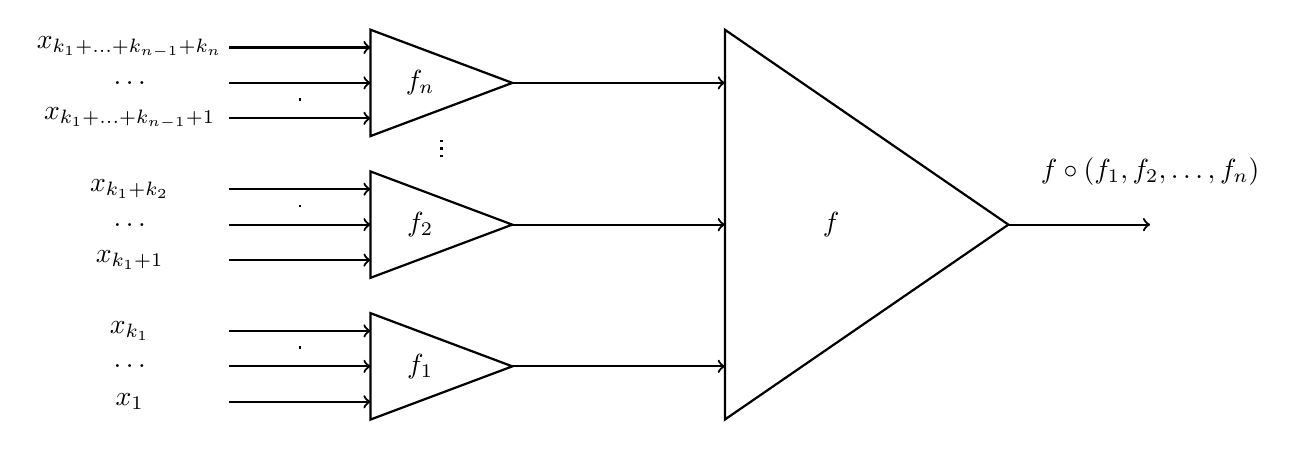
\begin{tikzpicture}[scale=0.9]
    % Main operation triangle
    \draw[thick, fill=white] (0,0) -- (0,5.5) -- (4,2.75) -- cycle;
    \node at (1.5,2.75) {$f$};

    % First sub-operation triangle
    \draw[thick, fill=white] (-5,0) -- (-5,1.5) -- (-3,0.75) -- cycle;
    \node at (-4.3,0.75) {$f_1$};

    % Second sub-operation triangle
    \draw[thick, fill=white] (-5,2) -- (-5,3.5) -- (-3,2.75) -- cycle;
    \node at (-4.3,2.75) {$f_2$};

    % Third sub-operation triangle (with dotted line indicating more)
    \draw[thick, fill=white] (-5,4) -- (-5,5.5) -- (-3,4.75) -- cycle;
    \node at (-4.3,4.75) {$f_n$};

    % Dotted line between second and third triangles
    \draw[dotted, thick] (-4,3.7) -- (-4,4);

    % Input arrows for first sub-operation
    \draw[->, thick] (-7,0.25) -- (-5,0.25);
    \draw[->, thick] (-7,0.75) -- (-5,0.75);
    \draw[->, thick] (-7,1.25) -- (-5,1.25);
    \node at (-8.4,0.25) {$x_1$};
    \node at (-8.4,0.75) {$\ldots$};
    \node at (-8.4,1.25) {$x_{k_1}$};

    % Input arrows for second sub-operation
    \draw[->, thick] (-7,2.25) -- (-5,2.25);
    \draw[->, thick] (-7,2.75) -- (-5,2.75);
    \draw[->, thick] (-7,3.25) -- (-5,3.25);
    \node at (-8.4,2.25) {$x_{k_1+1}$};
    \node at (-8.4,2.75) {$\ldots$};
    \node at (-8.4,3.25) {$x_{k_1+k_2}$};

    % Input arrows for third sub-operation
    \draw[->, thick] (-7,4.25) -- (-5,4.25);
    \draw[->, thick] (-7,4.75) -- (-5,4.75);
    \draw[->, thick] (-7,5.25) -- (-5,5.25);
    \node at (-8.4,4.25) {$x_{k_1+...+k_{n-1}+1}$};
    \node at (-8.4,4.75) {$\ldots$};
    \node at (-8.4,5.25) {$x_{k_1+...+k_{n-1}+k_n}$};

    % Connecting arrows from sub-operations to main operation
    \draw[->, thick] (-3,0.75) -- (0,0.75);
    \draw[->, thick] (-3,2.75) -- (0,2.75);
    \draw[->, thick] (-3,4.75) -- (0,4.75);

    % Output arrow
    \draw[->, thick] (4,2.75) -- (6,2.75);

    % Final output label
    \node at (6,3.5) {$f \circ (f_1, f_2, \ldots, f_n)$};

    % Dotted lines to indicate more inputs for each sub-operation
    \draw[dotted, thick] (-6,1) -- (-6,1.1);
    \draw[dotted, thick] (-6,3) -- (-6,3.1);
    \draw[dotted, thick] (-6,4.5) -- (-6,4.6);

\end{tikzpicture}
\caption{Operadic composition showing how multiple operations $f_1, f_2, \ldots, f_n$ with arities $k_1, k_2, \ldots, k_n$ can be composed with an operation $f$ of arity $n$ to form a new operation of arity $k_1 + k_2 + \ldots + k_n$.}
\label{fig:operadic-composition}
\end{figure}

Associativity of this composition for Operads works as follows:

\begin{figure}[h]
\centering
    \begin{tikzpicture}[grow'=up]
    \begin{scope}[xshift=-5cm]
        \node {(ab)c}
        child {
            node {ab}
            child {
                node {a}
            }
            child {
                node {b}
            }
        }
        child{
            node {c}
        };
    \end{scope}
    \begin{scope}[xshift=0cm]
        \node {(ab)c}
        child{
            node {a}
        }
        child {
            node {bc}
                child {
            node {b}
            }
            child {
                node {c}
            }
        };
    \end{scope}
    \begin{scope}[xshift=5cm]
        \node {abc}
        child{
            node {a}
        }
        child {
            node {b}
        }
        child {
            node {c}
        };
    \end{scope}
\end{tikzpicture}
    \caption{Associativity of operadic composition of arity 3}
\end{figure}

\begin{figure}[h]
\centering
\begin{tikzpicture}[grow'=up, level distance=1.5cm, sibling distance=2cm]
    % First tree: ((ab)c)d
    \begin{scope}[xshift=-10cm]
        \node {((ab)c)d}
        child {
            node {(ab)c}
            child {
                node {ab}
                child {
                    node {a}
                }
                child {
                    node {b}
                }
            }
            child {
                node {c}
            }
        }
        child {
            node {d}
        };
    \end{scope}

    % Second tree: (a(bc))d
    \begin{scope}[xshift=-5cm]
        \node {(a(bc))d}
        child {
            node {a(bc)}
            child {
                node {a}
            }
            child {
                node {bc}
                child {
                    node {b}
                }
                child {
                    node {c}
                }
            }
        }
        child {
            node {d}
        };
    \end{scope}

    % Third tree: (ab)(cd)
    \begin{scope}[yshift=6cm, xshift=0cm]
        \node {(ab)(cd)}
        child {
            node {ab}
            child {
                node {a}
            }
            child {
                node {b}
            }
        }
        child {
            node {cd}
            child {
                node {c}
            }
            child {
                node {d}
            }
        };
    \end{scope}

    % Fourth tree: a((bc)d)
    \begin{scope}[yshift=6cm, xshift=-10cm]
        \node {a((bc)d)}
        child {
            node {a}
        }
        child {
            node {(bc)d}
            child {
                node {bc}
                child {
                    node {b}
                }
                child {
                    node {c}
                }
            }
            child {
                node {d}
            }
        };
    \end{scope}

    % Fifth tree: a(b(cd))
    \begin{scope}[yshift=6cm, xshift=-5cm]
        \node {a(b(cd))}
        child {
            node {a}
        }
        child {
            node {b(cd)}
            child {
                node {b}
            }
            child {
                node {cd}
                child {
                    node {c}
                }
                child {
                    node {d}
                }
            }
        };
    \end{scope}

    \begin{scope}
        \node {abcd}
        child {
            node {a}
        }
        child {
            node {b}
        }
        child {
            node {c}
        }
        child {
            node {d}
        };
    \end{scope}

\end{tikzpicture}
\caption{Associativity of operadic composition of arity 4}
\label{fig:arity-4-associativity}
\end{figure}

This composition operation $\circ$ satisfies the following properties:

\begin{itemize}
  \item \textbf{Associativity}: For all $f \in \mathbb{P}(n)$, $g \in \mathbb{P}(k_1)$, $h \in \mathbb{P}(k_2)$, and $i \in \mathbb{P}(k_3)$, we have:

  \begin{equation}
    f \circ (g \circ (h, i)) = (f \circ (g, h)) \circ i
  \end{equation}

  \item \textbf{Unitality}: For all $f \in \mathbb{P}(n)$, we have:

  \begin{equation}
    f \circ (\text{id}_{k_1}, \text{id}_{k_2}, \ldots, \text{id}_{k_n}) = f
  \end{equation}

  where $\text{id}_k$ is the identity function on $\mathbb{X}^k$.
\end{itemize}

Symmetry is not required for operads, but it can be added to form symmetric operads. The symmetry condition is:

\begin{equation}
  f \circ (g_1, g_2, \ldots, g_n) = f \circ (g_{\sigma(1)}, g_{\sigma(2)}, \ldots, g_{\sigma(n)})
\end{equation}

where $\sigma$ is a permutation of the set $\{1, 2, \ldots, n\}$ or $\sigma \in S_n$ and $g_{\sigma(i)}$ is the $\sigma(i)$-th element of the original sequence, i.e., the permutation $\sigma$ permutes the order of operations used as inputs to $f$.

\subsubsection{Operads for Modeling}

Operads have been applied to modeling systems from diverse fields. In \textbf{physics}, operads have been extensively applied to model quantum field theories, where they capture the structure of Feynman diagrams and the composition of quantum interactions \cite{baez1997higher}. Operads of wiring diagrams have been used to model electrical circuits petri nets and quantum circuits \cite{spivak2013categorical, baez2020network}. Operads have also been employed in \textbf{computer science} to model SQL database query languages \cite{spivak2013categorical}, in \textbf{systems design} for modeling complex system design specification, analysis and synthesis \cite{behr2021operad}.

\subsection{Operads of Wiring Diagrams}

Wiring diagram operads provide a categorical framework for modeling directed compositional systems with explicit input-output interfaces \cite{spivak2013categorical,behr2021operad}. Unlike classical operads that focus purely on arity, wiring diagram operads encode both the connectivity structure and the directional flow of information through systems, making them particularly suited for modeling complex systems with hierarchical organization and modular decomposition.

\subsubsection{Formal Definition}

A wiring diagram operad $\mathcal{W}$ consists of graphical representations where operations are depicted as boxes with labeled input and output ports, connected by wires that carry typed information. Formally, we define:

\textbf{Wiring Diagrams:} A wiring diagram $W$ over a finite set of types $T$ is a directed graph where:
\begin{itemize}
    \item Vertices represent operations (boxes) with labeled input ports $\text{in}(v) \subseteq T$ and output ports $\text{out}(v) \subseteq T$
    \item Edges represent wires connecting output ports to input ports
    \item External inputs and outputs form the interface of the diagram
\end{itemize}

\textbf{Operations:} For a wiring diagram $W$ with input interface $I \subseteq T$ and output interface $O \subseteq T$, we denote the set of operations as $\mathcal{W}(I; O)$. Each operation $f \in \mathcal{W}(I; O)$ represents a morphism:

\begin{equation}
    f: \prod_{i \in I} X_i \to \prod_{o \in O} X_o
\end{equation}

where $X_t$ denotes the data type associated with type $t \in T$.

\begin{figure}[h]
\centering
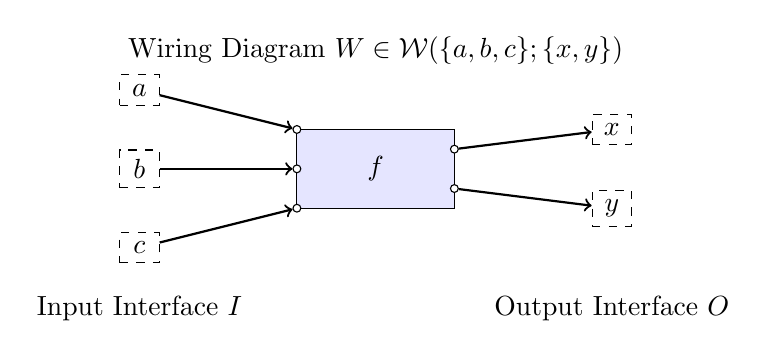
\begin{tikzpicture}[
  box/.style={rectangle, draw, minimum width=2cm, minimum height=1cm, fill=blue!10},
  wire/.style={->, thick},
  port/.style={circle, draw, fill=white, inner sep=1pt},
  interface/.style={rectangle, draw, dashed, minimum width=0.5cm, minimum height=0.3cm}
]

% Input interface
\node[interface] (in1) at (-3, 1) {$a$};
\node[interface] (in2) at (-3, 0) {$b$};
\node[interface] (in3) at (-3, -1) {$c$};

% Operation box
\node[box] (op1) at (0, 0) {$f$};

% Output interface  
\node[interface] (out1) at (3, 0.5) {$x$};
\node[interface] (out2) at (3, -0.5) {$y$};

% Input ports on box
\node[port] (p1) at (-1, 0.5) {};
\node[port] (p2) at (-1, 0) {};
\node[port] (p3) at (-1, -0.5) {};

% Output ports on box
\node[port] (q1) at (1, 0.25) {};
\node[port] (q2) at (1, -0.25) {};

% Wires
\draw[wire] (in1) -- (p1);
\draw[wire] (in2) -- (p2);
\draw[wire] (in3) -- (p3);
\draw[wire] (q1) -- (out1);
\draw[wire] (q2) -- (out2);

% Labels
\node[above] at (0, 1.2) {Wiring Diagram $W \in \mathcal{W}(\{a,b,c\}; \{x,y\})$};
\node[below] at (-3, -1.5) {Input Interface $I$};
\node[below] at (3, -1.5) {Output Interface $O$};

\end{tikzpicture}
\caption{Basic wiring diagram showing an operation $f$ with input interface $\{a,b,c\}$ and output interface $\{x,y\}$. Boxes represent operations, circles represent ports, and arrows represent typed wires.}
\label{fig:wiring-diagram-basic}
\end{figure}

\subsubsection{Composition Structure}

The composition operation in wiring diagram operads is defined through \textbf{substitution} and \textbf{wire connecting}. Given:
\begin{itemize}
    \item A wiring diagram $f \in \mathcal{W}(I; O)$ with input interface $I$ and output interface $O$
    \item Wiring diagrams $g_1 \in \mathcal{W}(I_1; O_1), g_2 \in \mathcal{W}(I_2; O_2), \ldots, g_k \in \mathcal{W}(I_k; O_k)$
\end{itemize}

The composition $f \circ (g_1, g_2, \ldots, g_k)$ is performed by:

\begin{enumerate}
    \item \textbf{Interface Matching:} Ensuring output interfaces of $g_i$ match corresponding input requirements in $f$
    \item \textbf{Diagram Substitution:} Replacing designated boxes in $f$ with the complete wiring diagrams $g_i$
    \item \textbf{Wire Connection:} Connecting output wires of $g_i$ to input wires of the corresponding positions in $f$
\end{enumerate}

The resulting composition has input interface $I' = \bigcup_{i=1}^k I_i$ and output interface $O$:

\begin{equation}
    f \circ (g_1, g_2, \ldots, g_k) \in \mathcal{W}\left(\bigcup_{i=1}^k I_i; O\right)
\end{equation}

\begin{figure}[h]
\centering
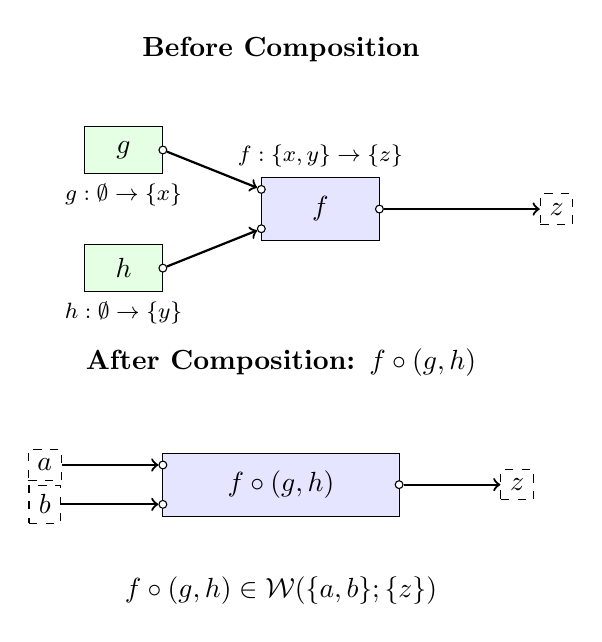
\begin{tikzpicture}[
  box/.style={rectangle, draw, minimum width=1.5cm, minimum height=0.8cm, fill=blue!10},
  subbox/.style={rectangle, draw, minimum width=1cm, minimum height=0.6cm, fill=green!10},
  wire/.style={->, thick},
  port/.style={circle, draw, fill=white, inner sep=1pt},
  interface/.style={rectangle, draw, dashed, minimum width=0.4cm, minimum height=0.25cm}
]

% Top diagram: Before composition
\node[above] at (0, 4.5) {\textbf{Before Composition}};

% Sub-operations g and h (Left side, outputs will feed into f)
\node[subbox] (g) at (-2, 3.5) {$g$};
\node[subbox] (h) at (-2, 2) {$h$};

% Main operation f (Receives outputs from g and h, centered relative to itself)
\node[box] (f) at (0.5, 2.75) {$f$};

% Output for f (Far right)
\node[interface] (out1) at (3.5, 2.75) {$z$};

% Ports for f (inputs left, output right)
\node[port] (fp1) at (-0.25, 3) {}; % Input from g
\node[port] (fp2) at (-0.25, 2.5) {}; % Input from h
\node[port] (fq) at (1.25, 2.75) {}; % Output z

% Ports for g
\node[port] (g_out) at (-1.5, 3.5) {};

% Ports for h  
\node[port] (h_out) at (-1.5, 2) {};

% Wires (Direct routing)
\draw[wire] (g_out) -- (fp1);
\draw[wire] (h_out) -- (fp2);
\draw[wire] (fq) -- (out1);

% Labels
\node[below, font=\footnotesize] at (g.south) {$g: \emptyset \to \{x\}$};
\node[below, font=\footnotesize] at (h.south) {$h: \emptyset \to \{y\}$};
\node[above, font=\footnotesize] at (f.north) {$f: \{x,y\} \to \{z\}$};

% Bottom diagram: After composition
\node[above] at (0, 0.5) {\textbf{After Composition: $f \circ (g, h)$}};

% Input interfaces for composed diagram (these are a and b)
\node[interface] (cin1) at (-3, -0.5) {$a$};
\node[interface] (cin2) at (-3, -1) {$b$};

% Composed operation box
\node[box, minimum width=3cm] (comp) at (0, -0.75) {$f \circ (g, h)$};

% Output
\node[interface] (cout) at (3, -0.75) {$z$};

% Ports
\node[port] (cp1) at (-1.5, -0.5) {};
\node[port] (cp2) at (-1.5, -1) {};
\node[port] (cq) at (1.5, -0.75) {};

% Wires  
\draw[wire] (cin1) -- (cp1);
\draw[wire] (cin2) -- (cp2);
\draw[wire] (cq) -- (cout);

% Result notation
\node[below] at (0, -1.8) {$f \circ (g, h) \in \mathcal{W}(\{a,b\}; \{z\})$};

\end{tikzpicture}
\caption{Composition of wiring diagrams showing how operations $g$ and $h$ are substituted into operation $f$. The top diagram shows the individual components, while the bottom shows the resulting composed operation.}
\label{fig:wiring-diagram-composition}
\end{figure}

\subsubsection{Associativity and Unitality}

Wiring diagram operads satisfy the fundamental operadic axioms:

\textbf{Associativity:} For compatible wiring diagrams, the composition operation is associative:
\begin{equation}
    (f \circ g) \circ h = f \circ (g \circ h)
\end{equation}

This corresponds to the fact that the order of substituting sub-diagrams does not affect the final connectivity structure.

\textbf{Unitality:} Identity wiring diagrams act as units under composition. For each type $t \in T$, there exists an identity operation $\text{id}_t \in \mathcal{W}(\{t\}; \{t\})$ that simply connects its input directly to its output:

\begin{equation}
    f \circ (\text{id}_{t_1}, \text{id}_{t_2}, \ldots, \text{id}_{t_n}) = f
\end{equation}

\subsubsection{Categorical Properties}

Wiring diagram operads form a \textbf{symmetric monoidal category} where:
\begin{itemize}
    \item Objects are finite sets of types (interfaces)
    \item Morphisms are wiring diagrams between interfaces
    \item Composition is given by diagram substitution
    \item The monoidal product corresponds to parallel composition of diagrams
    \item Symmetry is given by wire permutation
\end{itemize}

This categorical structure enables the modeling of complex systems with multiple subsystems operating in parallel, hierarchical decomposition through nested composition, and modular design patterns where components can be independently developed and later integrated.

\begin{figure}[h]
\centering
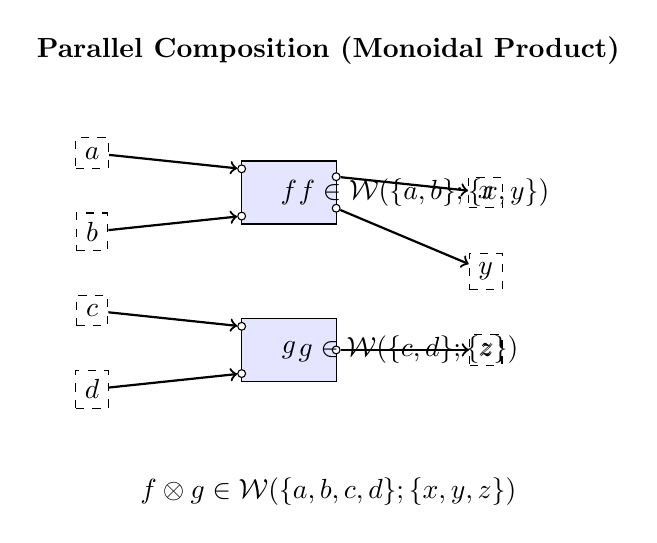
\begin{tikzpicture}[
  box/.style={rectangle, draw, minimum width=1.2cm, minimum height=0.8cm, fill=blue!10},
  wire/.style={->, thick},
  port/.style={circle, draw, fill=white, inner sep=1pt},
  interface/.style={rectangle, draw, dashed, minimum width=0.4cm, minimum height=0.25cm}
]

% Parallel composition demonstration
\node[above] at (0, 3) {\textbf{Parallel Composition (Monoidal Product)}};

% Input interfaces
\node[interface] (in1) at (-3, 2) {$a$};
\node[interface] (in2) at (-3, 1) {$b$};
\node[interface] (in3) at (-3, 0) {$c$};
\node[interface] (in4) at (-3, -1) {$d$};

% Two parallel operations
\node[box] (f) at (-0.5, 1.5) {$f$};
\node[box] (g) at (-0.5, -0.5) {$g$};

% Output interfaces
\node[interface] (out1) at (2, 1.5) {$x$};
\node[interface] (out2) at (2, 0.5) {$y$};
\node[interface] (out3) at (2, -0.5) {$z$};

% Ports for f
\node[port] (fp1) at (-1.1, 1.8) {};
\node[port] (fp2) at (-1.1, 1.2) {};
\node[port] (fq1) at (0.1, 1.7) {};
\node[port] (fq2) at (0.1, 1.3) {};

% Ports for g
\node[port] (gp1) at (-1.1, -0.2) {};
\node[port] (gp2) at (-1.1, -0.8) {};
\node[port] (gq) at (0.1, -0.5) {};

% Wires
\draw[wire] (in1) -- (fp1);
\draw[wire] (in2) -- (fp2);
\draw[wire] (in3) -- (gp1);
\draw[wire] (in4) -- (gp2);
\draw[wire] (fq1) -- (out1);
\draw[wire] (fq2) -- (out2);
\draw[wire] (gq) -- (out3);

% Labels
\node[right] at (f) {$f \in \mathcal{W}(\{a,b\}; \{x,y\})$};
\node[right] at (g) {$g \in \mathcal{W}(\{c,d\}; \{z\})$};

% Parallel composition notation
\node[below] at (0, -2) {$f \otimes g \in \mathcal{W}(\{a,b,c,d\}; \{x,y,z\})$};

\end{tikzpicture}
\caption{Parallel composition in wiring diagram operads demonstrating the monoidal product structure. Two operations $f$ and $g$ operate independently in parallel, with their interfaces combined disjointly.}
\label{fig:wiring-diagram-parallel}
\end{figure}
